\documentclass[a4paper,13pt,3p,twoside]{report} %twoside
\usepackage{scrextend}
\changefontsizes{13pt}
\usepackage[utf8]{vietnam}
\usepackage[top=2cm, bottom=2cm, left=3.5cm, right=2.5cm]{geometry}

\usepackage{graphicx} % Cho phép chèn hỉnh ảnh
\usepackage{fancybox} % Tạo khung box
\usepackage{indentfirst} % Thụt đầu dòng ở dòng đầu tiên trong đoạn
\usepackage{amsthm} % Cho phép thêm các môi trường định nghĩa
\usepackage{latexsym} % Các kí hiệu toán học
\usepackage{amsmath} % Hỗ trợ một số biểu thức toán học
\usepackage{amssymb} % Bổ sung thêm kí hiệu về toán học
\usepackage{amsbsy} % Hỗ trợ các kí hiệu in đậm
\usepackage{times} % Chọn font Time New Romans
\usepackage{array} % Tạo bảng array
\usepackage{enumitem} % Cho phép thay đổi kí hiệu của list
\usepackage{subfiles} % Chèn các file nhỏ, giúp chia các chapter ra nhiều file hơn
\usepackage{titlesec} % Giúp chỉnh sửa các tiêu đề, đề mục như chương, phần,..
\usepackage{titletoc}
\usepackage{chngcntr} % Dùng để thiết lập lại cách đánh số caption,..
\usepackage{pdflscape} % Đưa các bảng có kích thước đặt theo chiều ngang giấy
\usepackage{afterpage}
\usepackage[ruled,vlined]{algorithm2e}  % Hỗ trợ viết các giải thuật
\usepackage{capt-of} % Cho phép sử dụng caption lớn đối với landscape page
\usepackage{multirow} % Merge cells
\usepackage{fancyhdr} % Cho phép tùy biến header và footer
% \usepackage[natbib,backend=biber,style=ieee]{biblatex} % Giúp chèn tài liệu tham khảo
\usepackage{appendix}

\usepackage[font=small,labelfont=bf]{caption}

\usepackage{listings}
\usepackage{float}
\usepackage{subcaption}
\usepackage{xurl}

\usepackage[nonumberlist, nopostdot, nogroupskip, acronym]{glossaries}
\usepackage{glossary-superragged}
\setglossarystyle{superraggedheaderborder}
\usepackage{setspace}
\usepackage{parskip}

% package content table
\usepackage{tocbasic}

\usepackage{blindtext}

\usepackage{pdfpages} % Chèn pdf vào thanh trang mới

\usepackage{threeparttable}

\usepackage{stackengine}


% ===================================================

\renewcommand{\bibname}{Danh_sach_tai_lieu_tham_khao} 
\usepackage[backend=bibtex,style=ieee]{biblatex}  %backend=biber is 'better'

\renewcommand\appendixname{PHỤ LỤC}
\renewcommand\appendixpagename{PHỤ LỤC}
\renewcommand\appendixtocname{PHỤ LỤC}


\addbibresource{Danh_sach_tai_lieu_tham_khao.bib} % chèn file chứa danh mục tài liệu tham khảo vào 

%\include{lstlisting} % Phần này cho phép chèn code và formatting code như C, C++, Python

%\makeglossaries
\makenoidxglossaries

% Danh mục thuật ngữ và từ viết tắt
\newglossaryentry{IoT}{
    type=\acronymtype,
    name={IoT},
    description={Internet of Things},
    user1={Mạng lưới vạn vật kết nối Internet},
}

\newglossaryentry{AWGN}{
    type=\acronymtype,
    name={AWGN},
    description={Additive White Gaussian Noise},
    user1={Nhiễu trắng cộng dạng Gauss},
}

\newglossaryentry{FPGA}{
    type=\acronymtype,
    name={FPGA},
    description={Field Programmable Gate Array},
    user1={Cổng logic dạng mảng có thể tái lập trình},
}

\newglossaryentry{RAM}{
    type=\acronymtype,
    name={RAM},
    description={Random Access Memory},
    user1={Bộ nhớ đọc ghi ngẫu nhiên},
}

\newglossaryentry{HDL}{
    type=\acronymtype,
    name={HDL},
    description={Hardware Description Language},
    user1={Ngôn ngữ mô tả phần cứng},
}

\newglossaryentry{CPU}{
    type=\acronymtype,
    name={CPU},
    description={Central Processing Unit},
    user1={Bộ xử lý trung tâm},
}

\newglossaryentry{GPU}{
    type=\acronymtype,
    name={GPU},
    description={Graphics Processing Unit},
    user1={Bộ xử lý đồ họa},
}

\newglossaryentry{ASIC}{
    type=\acronymtype,
    name={ASIC},
    description={Application-Specific Integrated Circuit},
    user1={Mạch tích hợp chuyên dụng},
}

\newglossaryentry{SoC}{
    type=\acronymtype,
    name={SoC},
    description={System on Chip},
    user1={Hệ thống trên một vi mạch},
}

\newglossaryentry{SDR}{
    type=\acronymtype,
    name={SDR},
    description={Software-Defined Radio},
    user1={Chuẩn vô tuyến định nghĩa bằng phần mềm},
}

\newglossaryentry{GPIO}{
    type=\acronymtype,
    name={GPIO},
    description={General-Purpose Input/Output},
    user1={Chân tín hiệu đa mục đích},
}

\newglossaryentry{LAN}{
    type=\acronymtype,
    name={LAN},
    description={Local Area Network},
    user1={Mạng máy tính nội bộ},
}

%\newglossaryentry{FIFO}{
%    type=\acronymtype,
%    name={FIFO},
%    description={First In First Out},
%    user1={Bộ đệm nhập trước xuất trước},
%}

\newglossaryentry{FSM}{
    type=\acronymtype,
    name={FSM},
    description={Finite State Machine},
    user1={Trạng thái máy hữu hạn},
}

\newglossaryentry{UVM}{
    type=\acronymtype,
    name={UVM},
    description={Universal Verification Methodology},
    user1={Phương pháp kiểm thử tổng quát},
}

\newglossaryentry{DUT}{
    type=\acronymtype,
    name={DUT},
    description={Design Under Test},
    user1={Thiết kế cần kiểm thử},
}

\newglossaryentry{LUT}{
    type=\acronymtype,
    name={LUT},
    description={Look-Up Table},
    user1={Bảng tra cứu},
}

\newglossaryentry{FF}{
    type=\acronymtype,
    name={FF},
    description={Flip Flop},
    user1={Mạch Flip Flop},
}

\newglossaryentry{LUTRAM}{
    type=\acronymtype,
    name={LUTRAM},
    description={Look-Up Table Random Access Memory},
    user1={Bộ nhớ đọc ghi ngẫu nhiên cấu tạo từ bảng tra cứu},
}

\newglossaryentry{BUFG}{
    type=\acronymtype,
    name={BUFG},
    description={Global Clock Buffer},
    user1={Bộ đệm đồng hồ toàn cục},
}

\newglossaryentry{Endec Server}{
    type=\acronymtype,
    name={Endec Server},
    description={Encoder-Decoder Server},
    user1={Server mã hóa/giải mã},
}

\newglossaryentry{SNR}{
    type=\acronymtype,
    name={SNR},
    description={Signal-to-Noise Ratio},
    user1={Tỷ lệ tín hiệu trên tạp âm},
}

\newglossaryentry{AMP}{
    type=\acronymtype,
    name={AMP},
    description={Asymmetric Multi-Processing},
    user1={Xử lý đa lõi không đối xứng},
}

% ===================================================


\fancypagestyle{plain}{
    \fancyhf{} % clear all header and footer fields
    \fancyfoot[RO, LE]{\thepage}
% remove all header/footer rules
\renewcommand{\headrulewidth}{0pt}
\renewcommand{\footrulewidth}{0pt}}

\setlength{\headheight}{10pt}

\def \TITLE{ĐỒ ÁN TỐT NGHIỆP}
\def \AUTHOR{VŨ TUẤN MINH}

% ===================================================
\titleformat{\chapter}[hang]{\centering\bfseries}{CHƯƠNG \thechapter.\ }{0pt}{}[]

\titleformat 
    {\chapter} % command
    [hang] % shape
    {\centering\bfseries} % format
    {CHƯƠNG \thechapter.\ } % label
    {0pt} %sep
    {} % before
    [] % after
\titlespacing*{\chapter}{0pt}{-20pt}{20pt}

\titleformat
    {\section} % command
    [hang] % shape
    {\bfseries} % format
    {\thechapter.\arabic{section}\ \ \ \ } % label
    {0pt} %sep
    {} % before
    [] % after
\titlespacing{\section}{0pt}{\parskip}{0.5\parskip}

\titleformat
    {\subsection} % command
    [hang] % shape
    {\bfseries} % format
    {\thechapter.\arabic{section}.\arabic{subsection}\ \ \ \ } % label
    {0pt} %sep
    {} % before
    [] % after
\titlespacing{\subsection}{30pt}{\parskip}{0.5\parskip}

\renewcommand\thesubsubsection{\alph{subsubsection}}
\titleformat
    {\subsubsection} % command
    [hang] % shape
    {\bfseries} % format
    {\alph{subsubsection}, \ } % label
    {0pt} %sep
    {} % before
    [] % after
\titlespacing{\subsubsection}{50pt}{\parskip}{0.5\parskip}

% \newcommand{\titlesize}{\fontsize{18pt}{23pt}\selectfont}
% \newcommand{\subtitlesize}{\fontsize{16pt}{21pt}\selectfont}
% \titleclass{\part}{top}
% \titleformat{\part}[display]
%   {\normalfont\huge\bfseries}{\centering}{20pt}{\Huge\centering}
% \titlespacing{\part}{0pt}{em}{1em}
% \titlespacing{\section}{0pt}{\parskip}{0.5\parskip}
% \titlespacing{\subsection}{0pt}{\parskip}{0.5\parskip}
% \titlespacing{\subsubsection}{0pt}{\parskip}{0.5\parskip}


% ===================================================
\usepackage{hyperref}
\hypersetup{pdfborder = {0 0 0}} %
\hypersetup{pdftitle={\TITLE},
	pdfauthor={\AUTHOR}}
	
\usepackage[all]{hypcap} % Cho phép tham chiếu chính xác đến hình ảnh và bảng biểu

\graphicspath{{figures/}{../figures/}} % Thư mục chứa các hình ảnh

\counterwithin{figure}{chapter} % Đánh số hình ảnh kèm theo chapter. Ví dụ: Hình 1.1, 1.2,..

\title{\bf \TITLE}
\author{\AUTHOR}

\setcounter{secnumdepth}{3} % Cho phép subsubsection trong report
% \setcounter{tocdepth}{3} % Chèn subsubsection vào bảng mục lục

\theoremstyle{definition}
\newtheorem{example}{Ví dụ}[chapter] % Định nghĩa môi trường ví dụ

\onehalfspacing
%Khoảng cách xuống dòng
\setlength{\parskip}{6pt}
%Lùi đầu dòng
\setlength{\parindent}{15pt}





% added for 3 column glossaries

\usepackage{array}   % For column formatting
\usepackage{longtable} % For multi-page glossaries

% Custom 3-column style based on superraggedheaderborder
\newglossarystyle{my3colstyle}{%
    \setglossarystyle{superraggedheaderborder} % Inherit base style
    \renewenvironment{theglossary}%
        {\begin{longtable}{@{} l  p{0.2\textwidth}  p{0.35\textwidth}  p{0.35\textwidth}  @{}}} % 4 columns with row index
        {\end{longtable}}%
    \renewcommand*{\glossaryheader}{%
        \bfseries STT & \bfseries Thuật ngữ & \bfseries Ý nghĩa Tiếng Anh & \bfseries Ý nghĩa Tiếng Việt \\ \hline\hline \endhead}%
    \renewcommand{\glossentry}[2]{%
        \stepcounter{glossaryrow}% Increment row counter
        \theglossaryrow & % Display row number
        \glstarget{##1}{\glossentryname{##1}} &
        \glossentrydesc{##1} &
        \glsentryuseri{##1} \\ \hline} % Vietnamese in user1
    \renewcommand*{\subglossentry}[3]{\glossentry{##2}{##3}}%
}

% Counter for glossary rows
\newcounter{glossaryrow}
\setcounter{glossaryrow}{0}







% =========================== BODY ===============
\begin{document}
% \newgeometry{top=2cm, bottom=2cm, left=2cm, right=2cm}
\subfile{Bia} % Phần bìa
% \restoregeometry

% ===================================================
%\pagenumbering{roman}
%\pagestyle{empty} % Header và footer rỗng
%\newpage
%\subfile{chapters/0_1_subject.tex}
\pagenumbering{gobble}
\newpage
\null
\newpage

\newpage
\pagenumbering{gobble}
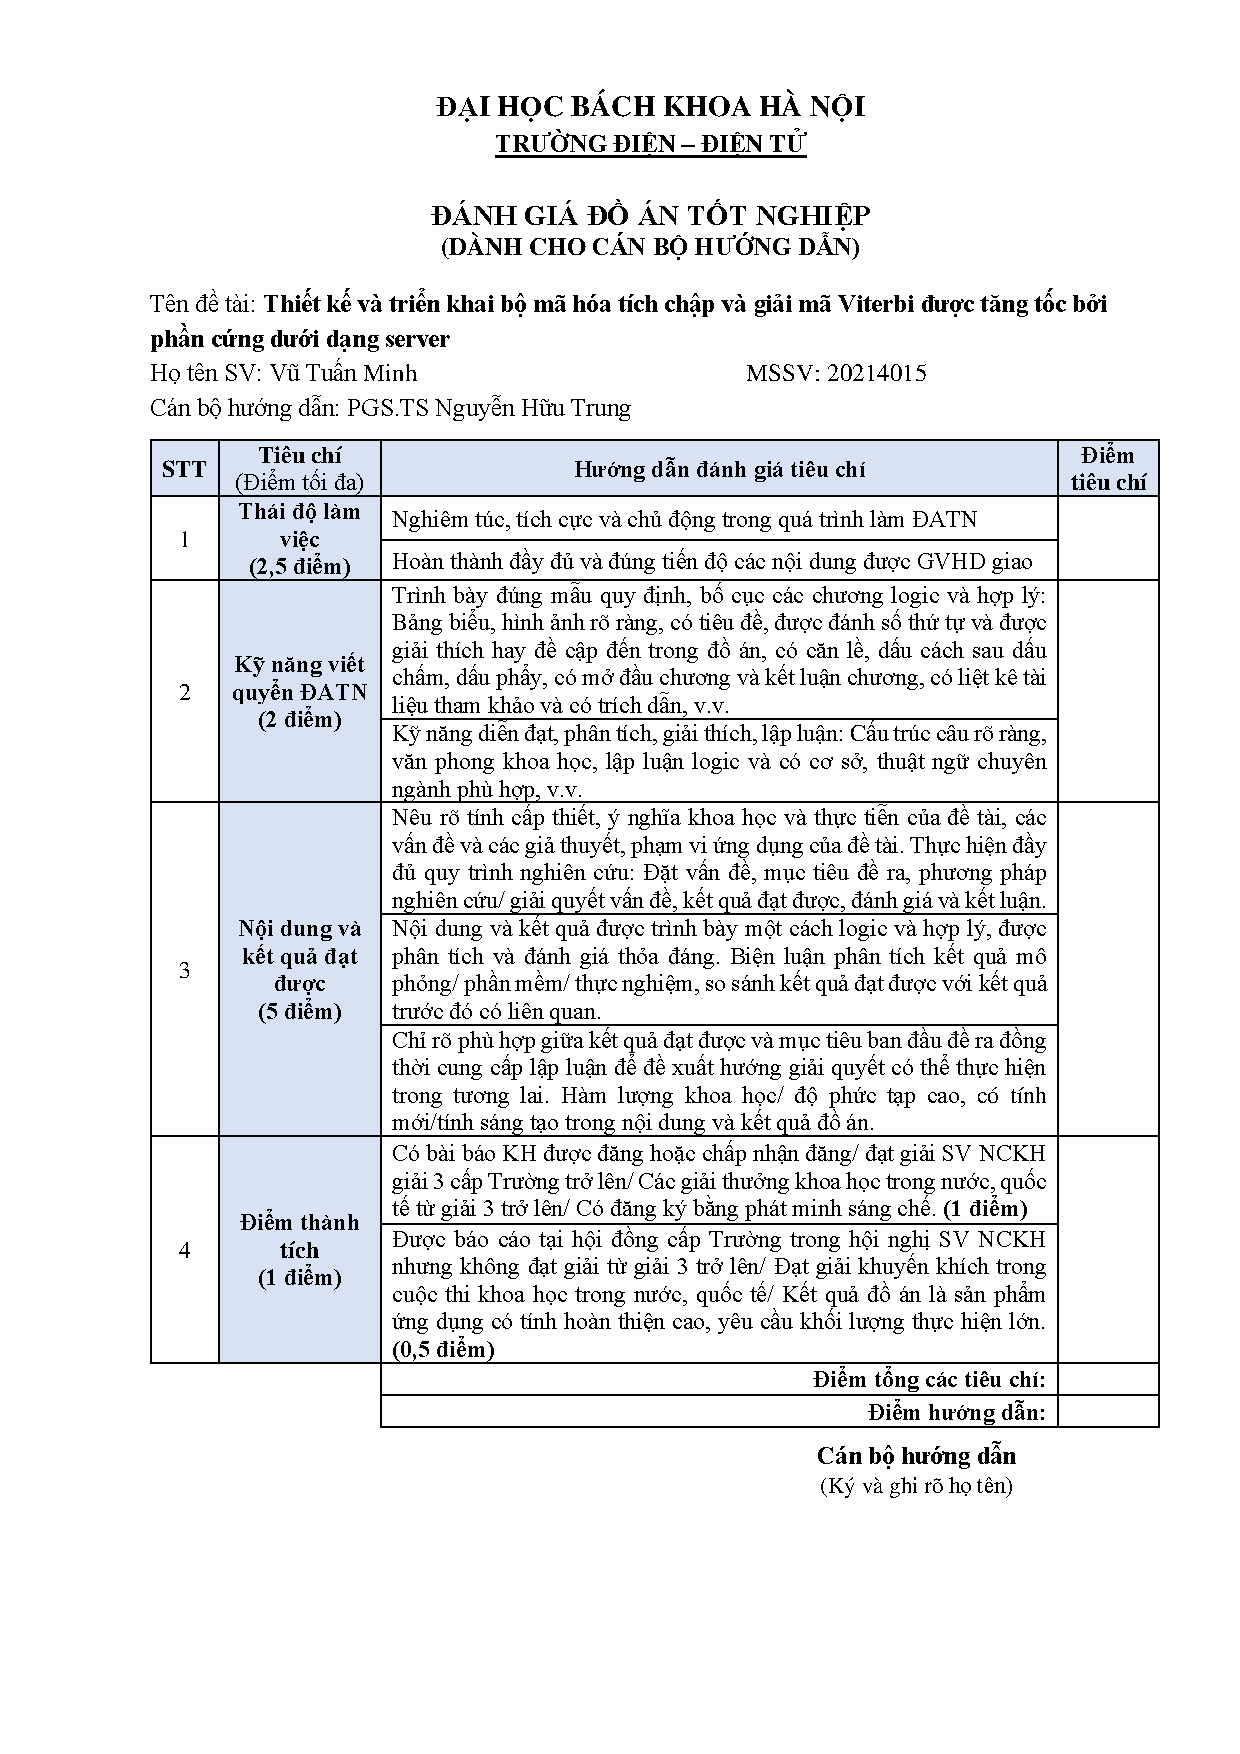
\includepdf[pages=-]{Phieu_Danh_Gia/Danh_gia_huong_dan.pdf}

\newpage
\null
\newpage

\newpage
\pagenumbering{gobble}
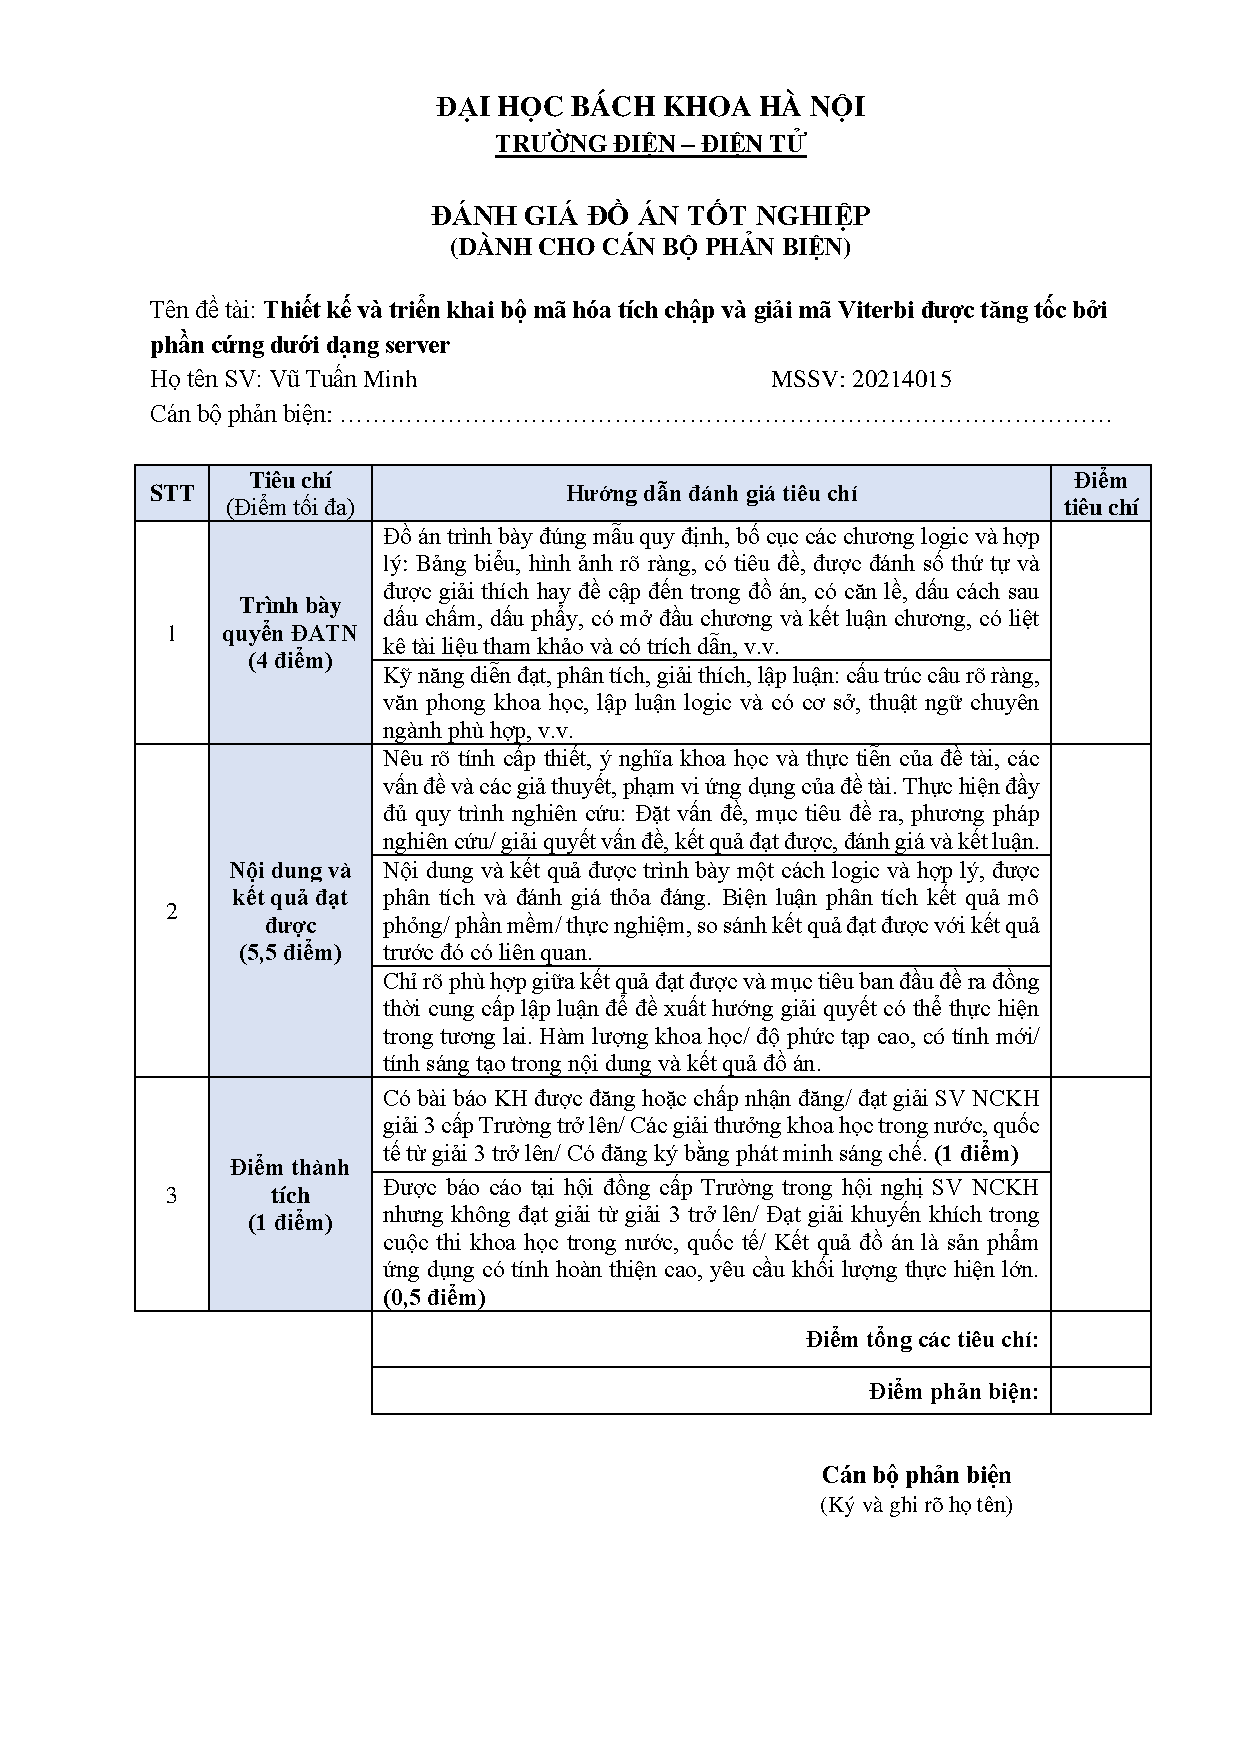
\includepdf[pages=-]{Phieu_Danh_Gia/Danh_gia_phan_bien.pdf}

\newpage
\null
\newpage

\newpage
\pagenumbering{gobble}
\subfile{Chuong/0_1_Loi_cam_ket.tex}

\newpage
\null
\newpage

\newpage
\pagenumbering{gobble}
\subfile{Chuong/0_2_Loi_cam_on.tex}

\newpage
\null
\newpage

\newpage
\pagenumbering{gobble}
\subfile{Chuong/0_3_Tom_tat_noi_dung.tex}

\newpage
\null
\newpage

%\newpage
%\pagenumbering{gobble}
%\subfile{Chuong/0_4_Tom_tat_noi_dung_English.tex}

% ===================================================
%\pagestyle{empty} % Header và footer rỗng
%\newpage
%\pagenumbering{roman} % Xóa page numbering ở cuối trang
\renewcommand*\contentsname{MỤC LỤC}

\titlecontents{chapter}
    [0.0cm]             % left margin
    {\bfseries\vspace{0.3cm}}                  % above code
    {{\bfseries{\scshape}
    CHƯƠNG \thecontentslabel.\ }}
    % numbered format
    {}         % unnumbered format
    {\titlerule*[0.3pc]{.}\contentspage}         % filler-page-format, e.g dots

    
\titlecontents{section}
    [0.0cm]             % left margin
    {\vspace{0.3cm}}                  % above code
    {\thecontentslabel \ } % numbered format
    {}         % unnumbered format
    {\titlerule*[0.3pc]{.}\contentspage}         % filler-page-format, e.g dots
    
\titlecontents{subsection}
    [1.0cm]             % left margin
    {\vspace{0.3cm}}                  % above code
    {\thecontentslabel \ } % numbered format
    {}         % unnumbered format
    {\titlerule*[0.3pc]{.}\contentspage}         % filler-page-format, e.g dots

 % Tạo mục lục tự động
\addtocontents{toc}{\protect\thispagestyle{empty}}
\tableofcontents 
\thispagestyle{empty}
%\cleardoublepage

%\pagenumbering{roman}
%Tạo danh mục hình vẽ.
\renewcommand{\listfigurename}{DANH MỤC HÌNH VẼ}
{\let\oldnumberline\numberline
\renewcommand{\numberline}{Hình~\oldnumberline}
\listoffigures} 
%\phantomsection\addcontentsline{toc}{section}{\numberline {} DANH MỤC HÌNH VẼ}
\newpage


 %Tạo danh mục bảng biểu.
\renewcommand{\listtablename}{DANH MỤC BẢNG BIỂU}
{\let\oldnumberline\numberline
\renewcommand{\numberline}{Bảng~\oldnumberline}
\listoftables}
% \phantomsection\addcontentsline{toc}{section}{\numberline {} DANH MỤC BẢNG BIỂU}

\setglossarystyle{my3colstyle} % Use our 3-column style
\glsaddall
\printglossary[title={Custom 3-Column Glossary}]



%\setlength{\glsdescwidth}{0.7\textwidth}

%\glsaddall 
\renewcommand*{\glossaryname}{Danh sách thuật ngữ}
\renewcommand*{\acronymname}{DANH MỤC THUẬT NGỮ}
\renewcommand*{\entryname}{Thuật ngữ}
\renewcommand*{\descriptionname}{Ý nghĩa}
\printnoidxglossaries
 %\phantomsection\addcontentsline{toc}{section}{\numberline {} DANH MỤC THUẬT NGỮ VÀ TỪ VIẾT TẮT}

\cleardoublepage

%\newpage
%\subfile{Chuong/0_5_Danh_muc_viet_tat}

%\newpage
%\subfile{Chuong/0_6_Thuat_ngu}
% ===================================================


\newpage
\pagenumbering{arabic}

% reset page numbering, careful for format when printing

\pagestyle{fancy}
\fancyhf{}
\fancyhead[RO, LE]{\leftmark} %RE, LO ; RO, LE
\fancyfoot[RO, LE]{\thepage}

\chapter{GIỚI THIỆU ĐỀ TÀI}
\label{chapter:Introduction}
\subfile{Chuong/1_Gioi_thieu} % Phần mở đầu

%\newpage
%\pagestyle{fancy} % Áp dụng header và footer
%\chapter{KHẢO SÁT VÀ PHÂN TÍCH YÊU CẦU}
%\label{chapter:Related_works}
%\subfile{Chuong/2_Khao_sat}


\newpage
%\pagestyle{fancy} % Áp dụng header và footer
\chapter{CƠ SỞ LÝ THUYẾT VÀ CÔNG NGHỆ SỬ DỤNG}
\label{chapter:Methodology}
\subfile{Chuong/3_Cong_nghe}

\newpage
%\pagestyle{fancy} % Áp dụng header và footer
\chapter{THIẾT KẾ, TRIỂN KHAI VÀ ĐÁNH GIÁ HỆ THỐNG}
\label{chapter:Experiment}
\subfile{Chuong/4_Ket_qua_thuc_nghiem}

%\newpage
%\pagestyle{fancy} % Áp dụng header và footer
%\chapter{CÁC GIẢI PHÁP VÀ ĐÓNG GÓP NỔI BẬT}
%\label{chapter:SolutionAndContribution}
%\subfile{Chuong/5_Giai_phap_dong_gop}


\newpage
%\pagestyle{fancy} % Áp dụng header và footer
\chapter{KẾT LUẬN} %Kết luận và hướng phát triển}
\label{chapter:conclusion}
\subfile{Chuong/6_Ket_luan}

%\newpage
%\pagestyle{fancy} % Áp dụng header và footer
%\chapter*{Lưu ý tài liệu tham khảo} %Kết luận và hướng phát triển}
%\label{chapter:reference}
%\subfile{Chuong/7_Luu_y_tai_lieu_tham_khao}


% ===================================================
\cleardoublepage
\newpage
\pagestyle{empty}
\pagenumbering{gobble}
\renewcommand\bibname{TÀI LIỆU THAM KHẢO}
\printbibliography
\phantomsection\addcontentsline{toc}{chapter}{TÀI LIỆU THAM KHẢO}

%\appendixpage % Tiêu đề phụ lục 
%\appendices
%\addappheadtotoc

% \chapter*{PHỤ LỤC} %Kết luận và hướng phát triển}

%\mainmatter
%\titleformat{\chapter}[hang]{\centering\bfseries}{ \thechapter.\ }{0pt}{}[]
%\titlespacing*{\chapter}{0pt}{-20pt}{20pt}

%\titlecontents{chapter}
%    [0.0cm]             % left margin
%    {\bfseries\vspace{0.3cm}}                  % above code
%    {{\bfseries{\scshape} \thecontentslabel.\ }} % numbered format
%    {}         % unnumbered format
%    {\titlerule*[0.3pc]{.}\contentspage}         % filler-page-format, e.g dots
%\chapter{HƯỚNG DẪN VIẾT ĐỒ ÁN TỐT NGHIỆP}
%\subfile{Chuong/Phu_luc_A}
%\newpage
%\chapter{ĐẶC TẢ USE CASE}
%\subfile{Chuong/Phu_luc_B}
\end{document}
